\section{SDepT v2.0.0概要}\label{sec:3}
%第3章ではSDepTの特徴やシステム構成, それぞれの手法の概要について書く
%開発言語やシステム構成の図などはここに.
%githubのURLもここに載せる予定

SDepT v2.0.0は,フロントエンドとバックエンドから構成される.
バックエンドは,統計解析に特化した開発実行環境を提供するR言語で開発されている.
しかし実際には,ある程度の統計解析の知識とプログラミングスキルがないと,R言語を用いて開発工数予測を行うことは難しい.
そこで,SDepT v2.0.0では、HTML,CSS,Java Scriptで実装されたユーザーフレンドリーなインターフェースを採用し,統計解析の数式やプログラミング言語に不慣れなユーザーでも利用できるようにした.

本研究で開発した開発工数予測ツールのシステム構成図を図1に示す.
図中の実践の部分はフロントエンド,点線の部分はバックエンドを示す.
また,バックエンドの背景のうち青色は前処理,緑色は複数工数予測手法の比較,橙色は新規プロジェクトの工数予測の処理を示している.(3.3節参照)
本システムは,フロントエンドとバックエンドから構成され,それぞれ\ref{subsec:3.1}節と\ref{subsec:3.2}節で詳しく述べる.
また,\ref{subsec:3.3}節では,それぞれの予測手法のについて具体的に述べる.
\begin{figure}[h]
  \centering
  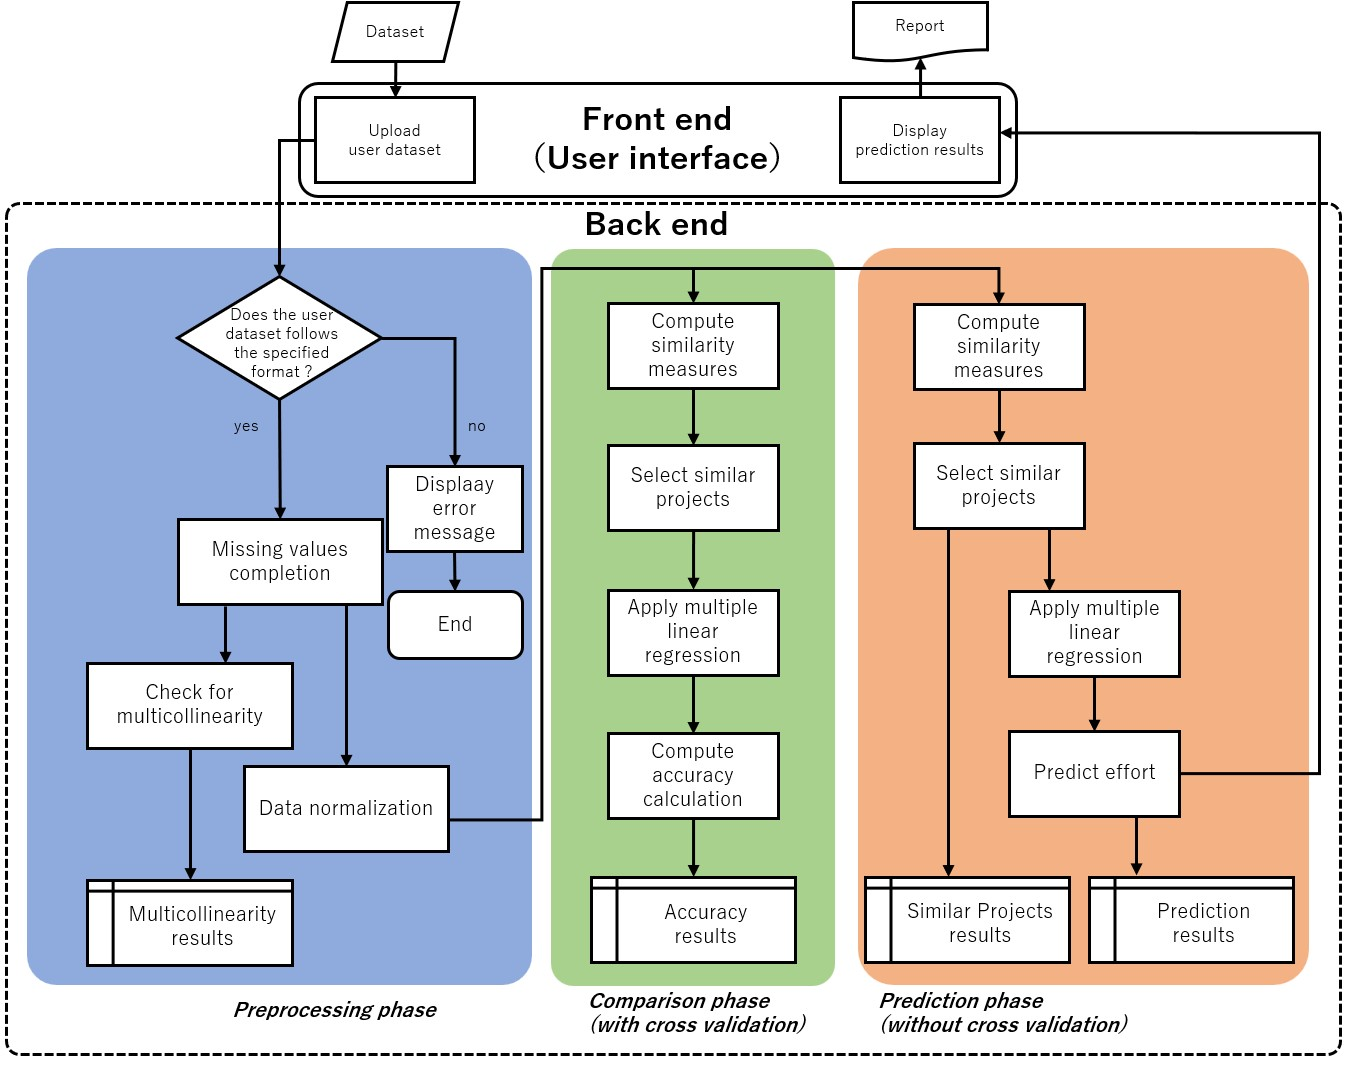
\includegraphics[width=120mm]{figure/fig/SystemArch_20241123.jpg}
  \captionsetup{labelformat=empty} % 図番号を非表示に設定
  \caption{\Fdualcaption{System Architecture of SDepT v2.0.0.}{SDepT v2.0.0 システム構成図.}}
  \label{fig:systemarch}
\end{figure}
% ラベルを英語にするのか日本語にするのか統一する

%%%%%%%%%%%%%%%%%%%%%%    3.1    %%%%%%%%%%%%%%%%%%%%%%
\clearpage
\subsection{フロントエンド}\label{subsec:3.1}
%フロントエンドの概要, 図も載せる予定
%現状フロントエンドの部分は去年と同じ
フロントエンドはHTML,CSS,Java Scriptを用いて実装している.
フロントエンドには2つのタブがあり,ユーザーは予備知識のレベルに応じて操作画面を選択することができる.
図\ref{fig:FrontBasic}および図\ref{fig:FrontAdvance}はそれぞれの操作画面であり,図\ref{fig:FrontBasic}はBasic画面,図\ref{fig:FrontAdvance}はAdvabce画面となっている.
1つ目のBasic画面では,ユーザーが精度と処理速度で重視する方を選択するのみで実行できるため,専門的な知識を必要としない.
一方,Advance画面では,ユーザーは各工程で用いる手法の選択が可能である.
さらに,類似プロジェクトの選定方法はそれぞれの$k$の値(それぞれの手法の類似プロジェクト選出範囲を調整できる(\ref{Selection}項参照))を選択できるため,より自由度の高い操作が可能となっている.手法を選択するため専門的な知識を要するが,選択した手法のみで実行できるため実行時間の短縮が期待できる.
どちらの画面においても,過去プロジェクトと新規プロジェクトのプロジェクト特性についてのデータセットをアップロードするが,必須項目は過去プロジェクトの開発工数のみである.
そのため,ユーザーが所有しているデータを最大限活用することができる.
予測結果は,csv形式のレポートとしてユーザーに返され,以下の項目が記載されている.
\begin{itemize}
  \item 各手法ごとの新規プロジェクトの開発工数予測値
  \item 各手法の予測精度
  \item 新規プロジェクトの類似プロジェクト
  \item VIF値
\end{itemize}

レポートを活用した開発工数の予測方法は,\ref{sec:4}で使用例を用いて解説する.
\begin{figure}[t]
  \centering
  % 左側の図
  \begin{minipage}[t]{0.49\textwidth}
      \centering
      \fbox{\includegraphics[width=0.9\textwidth]{figure/fig/Frontend_Basic.pdf}} % 左の画像
      \captionsetup{labelformat=empty} % 図番号を非表示に設定
      \caption{\Fdualcaption{“Basic” Tab of User interface.}{Basic画面のユーザインターフェース.}}
      \label{fig:FrontBasic}
  \end{minipage}
  \hfill
  % 右側の図
  \begin{minipage}[t]{0.49\textwidth}
      \centering
      \fbox{\includegraphics[width=0.9\textwidth]{figure/fig/Frontend_Advance.pdf}} % 右の画像
      \captionsetup{labelformat=empty} % 図番号を非表示に設定
      \caption{\Fdualcaption{“Advance” Tab of User interface.}{Advance画面のユーザインターフェース.}}
      \label{fig:FrontAdvance}
  \end{minipage}
\end{figure}
% コメント参照、ページのボトムに図を配置する

%%%%%%%%%%%%%%%%%%%%%%    3.2    %%%%%%%%%%%%%%%%%%%%%%
% 全部書いて見ないとわからないけど、次のページ行ってもいいかも
% \clearpage
\subsection{バックエンド}\label{subsec:3.2}
バックエンドはR言語を用いて実装している.
本節では,\ref{Preprocess}項で前処理,\ref{PastPrediction}項で複数工数予測手法の比較,\ref{NewPrediction}項で新規プロジェクトの工数予測の処理について詳しく述べる.
\subsubsection{前処理}\label{Preprocess}
%前処理について
前処理は主に4つの工程に分かれる.
\begin{enumerate}[label=前処理(\arabic*), leftmargin=6.0em]
  \item アップロードされたデータセットが以下の所定書式に沿っているか判定する.
  \begin{itemize}
    \item 1列目にプロジェクト番号が含まれているか.
    \item データセットの値が全て数値で入力されているか.
    \item 開発工数の列名が「Effort」となっているか.
    \item 新規プロジェクトのデータが最終行に格納されており目的変数がNULLとなっているか.
  \end{itemize}
  所定書式に沿っていない場合は操作画面にエラーメッセージが表示され,処理が終了する.
  \item データセットに欠損値が含まれていた場合,欠損値の補完をする.
  SDepT v2.0.0では欠損値の補完手法として,中央値補完,平均値補完,最頻値補完,$k$最近傍補完の4手法を採用している.(\ref{Imputation}項参照)
  \item 過去プロジェクトの説明変数間の多重共線性の有無を確認する.
  多重共線性とは,説明変数間で相関係数が高い組み合わせが存在することをいう.
  多重共線性が認められた場合,回帰係数が異常値になり回帰の精度に悪影響を及ぼす可能性がある.
  多重共線性は検出指標または分散拡大要因と呼ばれる VIF (Variance Inflation Factor) 値で判断できる.
  VIF値は式\ref{VIF}により算出する.
  \begin{equation}
    \label{VIF}
    VIF_{i}=  \frac{1}{(1 - R_{i}^{2} )}
  \end{equation}
  \begin{center}
  $i:$ 説明変数の個数$R_{i}:$ 回帰係数
  \end{center}
  $R_{i}^{2}$はVIFを求めたいデータセットの説明変数$x_{i}$を目的変数とし,その他の説明変数を説明変数として回帰した際の決定係数である.
  一般的にVIF \textgreater 10の場合に説明変数間に多重共線性があると判定を行う.
  これはVIF = 10であるなら相関係数に換算すると約 0.95 であり2変数の関連性が非常に強いことを意味するからである.
  \item 全ての特徴が同じ程度の影響度を持つように,データセットを正規化する.
  SDepT v2.0.0では正規化手法として,Huangら\cite{Huang2017}が比較していた3手法(Z-score,Min-Max[0,1],Min-Max[-1,1])に加え回帰分析によく使われる正規化手法の一つであるBox-Cox変換の計4手法を採用している.(\ref{Normalization}項参照 )
  以降の複数工数予測手法の比較や新規プロジェクトの工数予測は,ここで正規化されたデータを用いている.
  
\end{enumerate}
\subsubsection{複数工数予測手法の精度比較}\label{PastPrediction}
複数工数予測手法の精度比較では,ハイブリッド回帰ベースの予測アプローチ\cite{Hybrid}が実装されている.
主に4つの工程に分かれる.
\begin{itemize}
  \item 過去プロジェクト同士の類似度の計算
  \item 類似プロジェクトの選定
  \item 回帰による予測プロジェクトの算出
  \item 予測精度の比較
\end{itemize}
上記の各工程では,複数の手法が用意されており,それらの組み合わせによって計288種類の手法の提供が可能である.
各プロジェクトデータにおいて各手法における予測精度を算出することで,ユーザー側で比較が可能になる.
また,本工程では精度比較の際にleave-one-out cross validation法\cite{Kohavi1995}を実装している.
上記の工程は以下の手順で進む.
\begin{enumerate}[label=(\arabic*)]
  \item データセットの過去プロジェクトの中から1つ選択し、仮予測プロジェクトとする.
  \item 仮予測プロジェクトとそれ以外の過去プロジェクトの類似度を算出する.
  \item 算出した類似度を小さい順に並び替え,類似プロジェクトの選定手法によって選出された過去プロジェクトを類似プロジェクトとする.
  \item 選出した類似プロジェクトを元に8種類の回帰を適用し,仮予測プロジェクトの開発工数の予測値を算出する.
  \item 全ての過去プロジェクトに対して(1)~(4)を繰り返し行う.
  \item 上記の工程で算出された予測値を元に,各手法の予測精度を評価する.
\end{enumerate}
\subsubsection{新規プロジェクトの工数予測}\label{NewPrediction}
新規プロジェクトこ工数予測では,複数工数予測手法の比較で実装した288種類の手法を用いて,新規プロジェクト開発工数を予測する.

%%%%%%%%%%%%%%%%%%%%%%    3.3    %%%%%%%%%%%%%%%%%%%%%%
\clearpage
% 表はsection 3.3.1の上かな
\subsection{開発工数予測手法}\label{subsec:3.3}
\begin{table}[h]
  \centering
  \captionsetup{labelformat=empty} % 図番号を非表示に設定
  \caption{\Tdualcaption{Comparison of SDepT v1.0.0 and SDepT v2.0.0.}{SDepT v1.0.0とSDepT v2.0.0の比較.}}
  \label{table:Comparison}
    \begin{tabular}{|l|c|c|}
      \hline
      ~ & SDepT v1.0.0 & SDepT v2.0.0 \\ \hline
      %%%%%%%%正規化手法%%%%%%%%
      \multirow{4}{*}{欠損値補完手法} & 中央値補完 & 中央値補完 \\
       & & 平均値補完 \\
       & & 最頻値補完 \\
       & & $k$最近傍補完 \\ \hline
      %%%%%%%%欠損値補完手法%%%%%%%%
      \multirow{4}{*}{正規化手法} & z-score法 & z-score法 \\
       & & MinMax[0, 1] \\
       & & MinMax[-1, 1] \\
       & & BoxCox法 \\ \hline
      %%%%%%%%特徴選択手法%%%%%%%%
      \multirow{8}{*}{回帰手法} & OLS & OLS \\
       & Ridge & Ridge \\
       & Lasso & Lasso \\
       & Elastic Net & Elastic Net \\
       & SCAD & SCAD \\
       & MCP & MCP \\
       & & Adaptive Lasso \\
       & & Non-Negative Garrote \\ \hline
    \end{tabular}
\end{table}
本節では,本ツールで実装した前処理手法及びハイブリッド予測手法\cite{Hybrid}について説明する.本節では,\ref{Imputation}項では欠損値の補完手法,\ref{Normalization}項では正規化手法,\ref{Distance}項では類似度計算手法,\ref{Selection}項では類似プロジェクトの選定手法,\ref{Regression}項では回帰手法,\ref{Evaluation}項では評価尺度に用いた手法について紹介する.
なお,SDepT v2.0.0はSDepT v1.0.0と比べ,欠損値補完手法,正規化手法,回帰手法が拡張されており,変更点を表\ref{table:Comparison}に示す.
% 図じゃなくてtexで表で書いた方が見やすいかも

\subsubsection{欠損値補完手法}\label{Imputation}
欠損値補完手法には4つの手法を採用している.
\paragraph{中央値補完 \quad \\}
中央値補完はデータの中央値で欠損値を補完する手法である.
中央値は外れ値の影響を受けにくく,数値データに適している.
\paragraph{平均値補完 \quad \\}
平均値補完はデータの平均値で欠損値を補完する手法である.
外れ値が存在する場合,平均値は影響を受けやすいが,欠損値を全体の分布に近づけることができる.
\paragraph{最頻値補完 \quad \\}
最頻値補完はデータの最頻値で欠損値を補完する方法である.
カテゴリデータや離散的な数値データに適しており,データの分布を反映しやすい.
%SDepT v2.0.0では連続的な数値データの処理を想定しているため,あまり適さない可能性がある.
\paragraph{$k$最近傍補完 \quad \\}
$k$最近傍補完は,欠損値を含むプロジェクトにより近いk個のデータの平均値や中央値で欠損値を補完する方法である.
プロジェクト同士の距離を計算するため,大量のデータでは効率が悪くなってしまう場合があるが,データの分布やパターンを活かした高度な補完が可能である.
SDepT v2.0.0においては,$k=5$とし,数値データの場合は平均値,カテゴリデータの場合は最頻値で補完される.

\subsubsection{正規化及び標準化手法}\label{Normalization}
% 基本的に式の後にカンマ、句読点をつける (OR学会の添削でシャオ先生が式の後にカンマ、句読点をつけるように添削してたはず)
正規化手法には4つの手法を採用している.
\paragraph{Z-score法 \quad \\}
Z-score法\cite{Huang2017}は,平均$0$,分散$1$にデータを標準化する手法であり,式(\ref{Z-score})のように標準化される.
\begin{equation}
  \label{Z-score}
  x'_{i,j} = \frac{x_{i,j} - \bar(X_j)}{std(X_j)}.
\end{equation}
\begin{center}
  $x_{i,j}$:$i$番目のプロジェクトの$j$番目の説明変数,$X_j$:$j$列目のデータ列,$std(X_j)$:$X_j$の標準偏差
\end{center}

\paragraph{Min-Max$\lbrack0, 1\rbrack$ \quad \\}
Min-Max$\lbrack0, 1\rbrack$\cite{Huang2017}は,データを$0$から$1$の範囲に正規化する手法であり,式(\ref{MinMax01})のように正規化される.
\begin{equation}
  \label{MinMax01}
  x'_{i,j} = \frac{x_{i,j} - \min(X_j)}{\max(X_j) - \min(X_j)}
\end{equation}
\begin{center}
  $x_{i,j}$:$i$番目のプロジェクトの$j$番目の説明変数,$X_j$:$j$列目のデータ列
\end{center}

\paragraph{Min-Max$\lbrack-1, 1\rbrack$ \quad \\}
Min-Max$\lbrack-1, 1\rbrack$\cite{Huang2017}は,データを$-1$から$1$の範囲に正規化する手法であり,式(\ref{MinMax-11})のように正規化される.
\begin{equation}
  \label{MinMax-11}
  x'_{i,j} = 2 \cdot \frac{x_{i,j} - \min(X_j)}{\max(X_j) - \min(X_j)} - 1
\end{equation}
\begin{center}
  $x_{i,j}$:$i$番目のプロジェクトの$j$番目の説明変数,$X_j$:$j$列目のデータ列
\end{center}

\paragraph{BoxCox \quad \\}
BoxCox法は,式(\ref{BoxCox})のように正規化される.
\begin{equation}
  \label{BoxCox}
  x'_{i,j} = 
    \begin{cases} 
    \frac{x_{i,j}^\lambda - 1}{\lambda} & \text{if } \lambda \neq 0 \\
    \ln(x_{i,j}) & \text{if } \lambda = 0
    \end{cases}
\end{equation}
\begin{center}
  $x_{i,j}$:$i$番目のプロジェクトの$j$番目の説明変数,$\lambda$:BoxCox変換におけるパラメータ
\end{center}
BoxCox変換は$\lambda$の値によって以下のように変換の性質が変わる.
\begin{itemize}
  \item $\lambda=1$:元のデータを保持
  \item $\lambda=0$:対数変換($ln(x)$)
  \item $\lambda<1$:外れ値を抑える
  \item $\lambda>1$:データのばらつきを強調
\end{itemize}

\subsubsection{類似度計算手法}\label{Distance}
類似度計算には3つの手法を採用している.
\paragraph{ユークリッド距離(Euclidean Distance; ED) \quad \\}
% 参考文献の順番が若い番号順になるようにする。
ユークリッド距離\cite{Dejaeger2012}\cite{Shepperd1997}は,CBRで最も多く用いられている類似度尺度である.
予測プロジェクト$a$と過去プロジェクト$p$のユークリッド距離$ED_{a,p}$は式(\ref{ED})によって求める.
\begin{equation}
  \label{ED}
  ED_{a,p} = \sqrt{\sum_{j=1}^{n}(x'_{a,j} - x'_{p,j})^2}
\end{equation}
\paragraph{重み付きユークリッド距離(Weighted Euclidean Distance; W\_ED) \quad \\}
重み付きユークリッド距離は,通常のユークリッド距離における各プロジェクト特性の差にプロジェクト特性ごとに異なる重みをかけることで,特定のプロジェクト特性の重要度を付与することを可能にしている.
重み付きユークリッド距離を定式化したものが式(\ref{W_ED})である.
ここで,予測プロジェクトは$a$,過去プロジェクトは$p$,重み付きユークリッド距離は$wED$とする.
プロジェクト特性ごとの重み$w_i$は,菅\cite{菅2017}が紹介しているカテゴリースコアの算出法を採用している.
\begin{equation}
  \label{W_ED}
  wED_{a,p} = \sqrt{\sum_{j=1}^{n}w_i・(x'_{a,j} - x'_{p,j})^2}
\end{equation}
\paragraph{コサイン類似度(Cosine Similarity; COS) \quad \\}
コサイン類似度は,2つのベクトルのなす角のコサイン値を算出することで類似度を測定する手法である.
2つのベクトルの内積を2つのベクトルの大きさで割ることで計算される(\ref{COS}).
%値が$-1\sim1$に正規化されるため,正規化していない数値を式(\ref{COS})に代入し類似度を算出する.
\begin{equation}
  \label{COS}
  COS_{a,p}=\frac{\sum_{j=1}^{m}x'_{a,j}・x'_{p,j}}{\sqrt{\sum_{j=1}^{m}(x'_{a,j})^2}\sqrt{\sum_{j=1}^{m}(x'_{p,j})^2}}
\end{equation}
\subsubsection{類似プロジェクト選定手法}\label{Selection}
類似プロジェクト選定には3つの手法を採用している.
\paragraph{クラスタリング \quad \\}
クラスタリング\cite{Hai2022}は異なる性質のものが混ざり合った集団から,互いに似た性質を持つものを集め,クラスタ (集合) をつくる方法である. クラスタ分析には様々な手法があるが,本研究では,非階層型クラスタ分析手法の一つでありソフトウェア開発労力の予測にも用いられている,$k$-means法を採用する.
% 階層型クラスタ分析はあらかじめ分割するクラスタの数を決める必要がなく, 結果の全体像を樹形図に表示できるため, 全体に対するサンプルの位置づけ, 形成されたクラスタ間の相対的な位置づけが比較できる. 一方, 非階層型クラスタ分析では, あらかじめクラスタの数を指定する必要があり, 全体像の解釈は困難である. 階層型の短所としては対象を一度分類すると分類が確定してしまうため, 信頼性が低い. それに対して非階層型は一度分類してもそれより適した分類になるまでクラスタ間を移動させるため, より自然で信頼性の高い分類が可能になる. 一般的な非階層型クラスタ分析の手法として, k-means法が代表的であり, ソフトウェア開発労力の予測にも用いられている. そこで, 本研究はk-means法を用いる.
一般的に$k$-means法は, 次のようにクラスタを生成する.
% 手順なら(1), (2)てきな感じで書く(他の手順の説明がこの表記で書かれているみたいだから)
\begin{enumerate}
  \item クラスタの核 (クラスタの中心) を$k$個仮定する.
  \item 核の位置が変化しなくなるまで以下を繰り返す.
  \begin{itemize}
    \item 各プロジェクトを最も距離の短い核のクラスタに分類する.
    \item 各クラスタに分類されたプロジェクトの平均を該当クラスタの新しい核とする.
  \end{itemize}
\end{enumerate}
本研究では,予測プロジェクトが含まれるクラスタに分類された過去プロジェクトを類似ブロジェクトとして選出する.
また,クラスタの数$k$はユーザ自身で設定が可能であり,デフォルトでは$k=2,3,4,5$としている.
\paragraph{Fixed-$k$ \quad \\}
Fixed-$k$では昇順にソートした類似度の,小さいものから$k$個を類似プロジェクトとして選定する.
$k$の取り方はユーザ自身で設定が可能であり,デフォルトでは$k=3,4,5,6$となっている.
\paragraph{四分位数法 \quad \\}
四分位数法は,Fixed-$k$と同様に類似度を昇順にソートし,四等分することで類似プロジェクトを選定する手法である.
以下の手順によって選定を行う.
\begin{enumerate}[label=(\arabic*)]
  \item 予測プロジェクトとの類似度を昇順にソートする
  \item 昇順にした類似度ベクトルを四等分する
  \item 四等分したもののうち,より類似度の近い集合$k$個を類似プロジェクトとして選定する
\end{enumerate}
ここでの$k$もユーザ自身が設定でき,デフォルトは$k=1,2,3,4$である.
分割パターンは全てFixed-$k$の分割パターンに含まれているが,全体に対して類似プロジェクトとして選定されている割合がイメージしやすいため採用している.
\subsubsection{回帰手法}\label{Regression}
一般的に,線形重回帰モデルは式(\ref{LMR})で表される.
\begin{equation}
  \label{LMR}
  Y_{i} = \sum_{j=0}^{n}{\beta_{j}X_{i,j}+\epsilon}
\end{equation}
ここで,$Y_{i}$と$X_{i,j}$はそれぞれ,プロジェクト$i~(i=1,~2,...,~m)$の開発工数とプロジェクト特性$j~(i=1,~2,...,~n)$を表す.また,$\beta_0,~\beta_1,~...,~\beta_n$は回帰係数であり,$\epsilon$は確率誤差項である.
正規化済みデータを用いて回帰を行い,回帰の後逆変換を施すことで予測値を算出する.
% このモデルは,誤差の平均が0,分散が一定であるという仮定の元に成り立つため,回帰を行う前に対数変換を行う.回帰ののちに逆対数変換の処理を施すことで予測値を算出する.
% また,回帰を行う前に対数変換を行い,回帰後の値に逆対数変換の処理を施すことで予測値を算出する.
%線形重回帰モデルを用いる際に,以下の4つの仮定を設ける.
%\begin{enumerate}[(仮定1)]
  %\item 誤差の平均値が0である. \\ $E[\epsilon]=0.$
  %\item 誤差の分散が一定である. \\ $Var[\epsilon]=\sigma^2.$
  %\item 各誤差は互いに独立であり,その共分散は0である. \\ $E[\epsilon_i \epsilon_i']=0, (i\neq i',~i=1,~2,~...,~m,~i'=1,~2,~...,~m)$
  %\item 誤差は以下のような正規確率密度関数に従う. \\ $p(z)=(2\pi\sigma^2)^(-1/2)\exp[z^2/2\sigma^2]$
%\end{enumerate}
%これらの仮定を満たすために回帰を行う前に対数変換を行い,回帰ののち逆対数変換の処理を施すことで予測値を算出する.
回帰には8つの手法を採用している.

\paragraph{最小二乗法(Ordinary Least Squares; OLS) \quad \\}
回帰係数を$\beta(\beta=\beta_0,\beta_1,...,\beta_m)$とし,OLSによる推定値$\hat{\beta}_{OLS}$は式(\ref{OLS})によって与えられる.
\begin{equation}
  \label{OLS}
  \bm{\hat{\beta}}_{OLS} = \underset{\bm{\beta}}{\arg min}\sum_{i=1}^{n}(y_{i} -\sum_{j=0}^{m}\beta_{j}x_{i,j})^2
\end{equation}
%ここで,説明変数には互いに強い相関を持つことが多く,多重共線性が存在する場合においてはOLSでの推定値が不安定になることが知られている.
%対策として,説明変数の選択を行うことが効果的である.
%目的変数に対して効果的である説明変数を残すために,本研究ではステップワイズ法を採用する.
%また,変数選択の評価尺度には赤池情報量基準(Akaike Infomation Criterion;AIC)\cite{AIC}を用いる.

\paragraph{Ridge回帰 \quad \\}
Ridge回帰\cite{Ridge}\cite{Araki2013}\cite{Hastie2009}は,罰則項がついている回帰手法である.
罰則項により,多重共線性に対処できる.
式(\ref{Ridge})によって算出され,式中の$\lambda\sum_{j=1}^{m}\beta_{j}^2$が罰則項である.
$\lambda$によって罰則項の強さが調整でき,$\lambda=0$のときOLSとなり,$\lambda$が大きいほど罰則が強くなる.
%また,Ridge回帰と後述のLasso回帰の制約領域の模式図を図\ref{fig:ridge_lasso}に示す.
\begin{equation}
  \label{Ridge}
  \bm{\hat{\beta}_{Ridge}} =\underset{\bm{\beta}}{\arg min}\lbrace\sum_{i=1}^{n}(y_{i} -\sum_{j=0}^{m}\beta_{j}x_{i,j})^2 +\lambda\sum_{j=1}^{m}\beta_{j}^2\rbrace
\end{equation}
%% \begin{figure}[h]
%   \centering
%   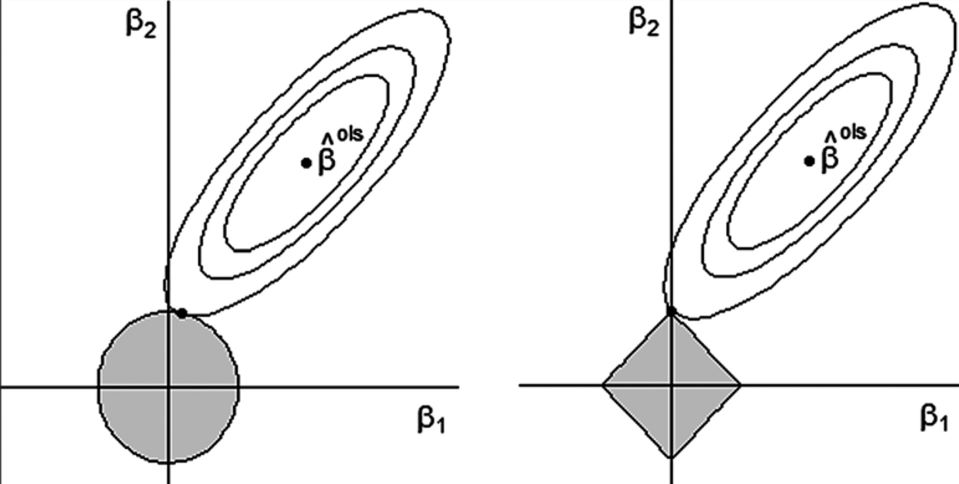
\includegraphics[width=120mm]{figures/fig/ridgelasso.jpg}
%   \caption{Ridge回帰とLasso回帰の制約領域の模式図\cite{RidgeLasso2}}
%   \label{fig:ridge_lasso}
% \end{figure}

\paragraph{Lasso回帰 \quad \\}
Lasso回帰\cite{Araki2013}\cite{Hastie2009}\cite{Tibshirani2018}は,Ridge回帰と同様,罰則項がついている回帰手法である.
Lasso回帰は式(\ref{Lasso})で算出される.
Ridge回帰と異なる点は,罰則項が$\lambda\sum_{j=1}^{m}|\beta_{j}|$となっている点である.
\begin{equation}
  \label{Lasso}
  \bm{\hat{\beta}_{Lasso}} =
\underset{\bm{\beta}}{\arg min}\lbrace\sum_{i=1}^{n}(y_{i} -\sum_{j=0}^{m}\beta_{j}x_{i,j})^2 +\lambda\sum_{j=1}^{m}|\beta_{j}|\rbrace
\end{equation}
\vskip\baselineskip

\paragraph{Elastic Net回帰 \quad \\}
ElasticNet回帰\cite{Zou2005}は,Ridge回帰とLasso回帰の罰則項をどちらも採用している回帰手法である.
式(\ref{Elastic})によって算出される.
\begin{equation}
  \label{Elastic}
  \bm{\hat{\beta}_{Elastic}} =
\underset{\bm{\beta}}{\arg min}\lbrace\sum_{i=1}^{n}(y_{i} -\sum_{j=0}^{m}\beta_{j}x_{i,j})^2 +\lambda\sum_{j=1}^{m}(\frac{1}{2}(1-\alpha)\beta_{j}^2+\alpha|\beta_{j}|)\rbrace
\end{equation}
\paragraph{SCAD回帰 \quad \\}
SCAD回帰\cite{Fan2001}は,Lasso回帰の拡張として提案された回帰手法である.
大きな係数に対してはLasso回帰,小さな係数に対してはRidge回帰の罰則項のような効果を持つという特徴がある.
式(\ref{SCAD})で算出でき,罰則項は式(\ref{SCAD_J})で与えられる.
\begin{equation}
  \label{SCAD}
  \bm{\hat{\beta}_{SCAD}} =\underset{\bm{\beta}}{\arg min}\lbrace\frac{1}{2}\sum_{i=1}^{n}(y_{i} -\sum_{j=0}^{m}\beta_{j}x_{i,j})^2 +\sum_{j=1}^{m}J(\beta_{j})\rbrace
\end{equation}
\begin{equation}
  \label{SCAD_J}
  J(\beta)=
  \begin{cases}
    \lambda|\beta| &(|\beta|\le\lambda) \\
    \frac{\beta^2-2a\lambda|\beta|+\lambda^2}{2(a-1)} &(\lambda<|\beta|\le a\lambda) \\
    \frac{(a+1)\lambda^2}{2} &(|\beta|>a\lambda)
  \end{cases}
\end{equation}
\paragraph{MCP回帰 \quad \\}
MCP (Multiple Change Points;MCP)回帰\cite{Zhang2010}は,SCAD回帰同様,Lasso回帰の拡張として提案された回帰手法である.
SCAD回帰よりも構造が簡単で,計算が容易であるという利点を持つ.
式(\ref{MCP})で算出でき,罰則項は式(\ref{MCP_J})で与えられる.
\begin{equation}
  \label{MCP}
  \bm{\hat{\beta}_{SCAD}} =\underset{\bm{\beta}}{\arg min}\lbrace\frac{1}{2}\sum_{i=1}^{n}(y_{i} -\sum_{j=0}^{m}\beta_{j}x_{i,j})^2 +\sum_{j=1}^{m}J(\beta_{j})\rbrace
\end{equation}
\begin{equation}
  \label{MCP_J}
  J(\beta)=
  \begin{cases}
    \lambda|\beta|-\frac{x^2}{2a} &(|\beta|\le a\lambda) \\
    \frac{a\lambda^2}{2} &(|\beta|>a\lambda)
  \end{cases}
\end{equation}

\paragraph{Adaptive Lasso回帰 \quad \\}
AdaptiveLasso回帰\cite{Zou2006}\cite{Araki2013}は2段階推定を行う回帰手法である.
第1段階で$\bm{\beta}$の初期推定量(本研究では$\bm{\hat{\beta}}_{ridge}$)を求め,第2段階で,式(\ref{AdaptiveWeight})を用いて算出した重み$\hat{\omega}_{j}$をペナルティとして課した罰則項付き回帰(式(\ref{AdaptiveLasso}))を行う.
なお,本研究では$\gamma=2$とした.
\begin{equation}
  \label{AdaptiveWeight}
  \hat{\omega}_{j}= 
  \begin{cases} 
  \frac{1}{|\bm{\beta}_{ridge.j}|^\gamma} & \text{where } \bm{\beta}_{ridge.j} \neq 0\\
  \inf & \text{where } \bm{\beta}_{ridge.j} = 0
  \end{cases}
\end{equation}
\begin{equation}
  \label{AdaptiveLasso}
  \bm{\hat{\beta}_{AdaptiveLasso}} =
\underset{\bm{\beta}}{\arg min}\lbrace\sum_{i=1}^{n}(y_{i} -\sum_{j=0}^{m}\beta_{j}x_{i,j})^2 +\lambda\sum_{j=1}^{m}\hat\omega_{j}|\beta_{j}|\rbrace
\end{equation}

\paragraph{Non-Negative Garrote回帰 \quad \\}
Non-NegativeGarrote回帰\cite{Zou2006}\cite{Araki2013}は,非負の因子である$c=(c_{1}, c_{2},\dots,c_m)$を用いて$\bm{\hat{\beta}}$の要素を直接縮小して推定する手法である.式(\ref{NonNegativeGarrote})で与えられる.
\begin{equation}
  \label{NonNegativeGarrote}
  \begin{split} 
  \bm{\hat{\beta}_{NonNegative}} =
  &\underset{\bm{\beta}}{\arg min}\lbrace\sum_{i=1}^{n}(y_{i} -\sum_{j=0}^{m}\bm{\beta}_{ols.j}x_{i,j}c_{j})^2 +\lambda\sum_{j=1}^{m}|c_{j}|\rbrace\\
  &c_{j}\geq0
  \end{split} 
\end{equation}

\subsubsection{評価尺度}\label{Evaluation}
評価尺度には4つの手法を採用している.
\paragraph{MMRE(Mean Magnitude of Relative Error) \quad \\}
MMREとはMREの平均値であり,MREは予測値と実測値との相対誤差を表す指標である.
プロジェクト$i$の開発工数値$y_{i}$と予測値$\hat{y_{i}}$の$MRE_{i}$は式(\ref{MRE})によって算出され,$MMRE$は式(\ref{MMRE})によって算出される.
数値が小さいほど予測精度が高いことを示す.
\begin{equation}
  \label{MRE}
  MRE_{i} = \frac{|y_{i}-\hat{y}_{i}|}{y_{i}}
\end{equation}
\begin{equation}
  \label{MMRE}
  MMRE = \frac{\sum_{i=1}^{n}MRE_{i}}{n}
\end{equation}
\paragraph{MdMRE(Median Magnitude of Relative Error) \quad \\}
MdMREはMREの中央値である.
MdMREはMREと同様に数値が小さいほど予測精度が高いことを示す.
\paragraph{Pred($p$) \quad \\}
Pred($p$)\cite{Port2008}は予測値と実測値のMREが$p$\%以下となった割合を示し,数値が大きいほど予測精度が高いことを示す.
本実験では,Pred($25$)と設定して開発を行う.
MREが25\%以下となったプロジェクトの件数を$s$と置くとPred($25$)は式(\ref{Pred})にて算出される.
\begin{equation}
  \label{Pred}
  Pred(25) = 100 \times \frac{s}{n}
\end{equation}
\paragraph{SA(Standardized Accuracy) \quad \\}
SA\cite{Shepperd2012}は,Predと同様に数値が大きいほど予測精度が高いことを示し,式(\ref{SA})で算出される.
また,$MAE$は$i$番目のプロジェクトの実測工数$y_i$とその予測値$\hat{y_i}$との誤差平均であり,式(\ref{MAE})で算出される.
$MAE_{0}$は$\hat{y}$の代わりに,$j$番目のプロジェクトの実測工数$y_j$をランダムに割り当てた場合の絶対誤差平均であり,式(\ref{MAE0})で算出される.
\begin{equation}
  \label{SA}
  SA =\Big(1 - \frac{MAE}{MAE_{p0}} \Big) \times 100
\end{equation}

\begin{equation}
  \label{MAE}
  MAE =\frac{1}{m} \sum_{i=1}^{m} |y_{i} - {\hat{y}_{i}}|
\end{equation}

\begin{equation}
  \label{MAE0}
  MAE_{p0} =\frac{2}{m^2} \sum_{i=1}^{m} \sum_{j=1}^{j<i} |y_{i} - y_{j}|
\end{equation}
